\chapter{Problémy a jejich řešení}
\label{7-problemy}

\section{Použití knihovny GEOS}
\label{problemy-geos}
Jako poměrně zásadní problém se ukázalo použití knihovny \textit{GEOS}. 
Přestože tato knihovna je napsána v~jazyku C++, obsahuje \textit{wrapper} 
v~podobě C~API. Hlavním důvodem toho je zajištění vyšší 
stability. Při~použití C~API totiž není nutné vlastní aplikaci,
která ho používá, při~každé změně v~knihovně \textit{GEOS} překompilovat. 
Proto většina programů využívajících \textit{GEOS} a~mezi nimi i~Quantum 
GIS používají právě C~API. Nicméně to má i~své nevýhody. V~C~API bohužel 
zatím není implementována veškerá funkcionalita C++~API. Některé chybějící 
funkce lze obejít aplikací sice složitějšího postupu, nicméně výsledek je 
obdobný jako při~použití C++~API. Avšak jiná funkcionalita je pro~uživatele 
C~API zcela nedostupná. Po~dlouhých úvahách\footnote{O~problému jsem napsala
na~\textit{mailing-list} vývojářů \textit{GEOSu} a~odpovědí bylo uvedení 
již zmíněných pro a~proti. Problém jsem následně prodiskutovala s~vedoucím 
práce, který mi doporučil toto řešení.} bylo proto v~knihovně \textit{GEOC} 
přistoupeno k~využití C++~API i~s~rizikem, že bude při~každé změně nutné 
vše překompilovat. %% ML: odkaz pod carou - odkaz na diskuzi ML  

S~tím souvisí i~další problém převodu geometrie. Jelikož v~programu QGIS je 
používáno právě C~API, nelze GEOS geometrii jednoduše převést na~typ QGIS 
geometrie. Tento problém byl vyřešen konverzí mezi těmito dvěma typy přes 
WKT\footnote{textový značkovací jazyk pro popis vektorové 
geometrie geografických objektů apod.}. Nevýhoda tohoto postupu je však 
zpomalení běhu programu obzvláště u~rozsáhlejších datasetů. Toto by mělo
být v~budoucnu vyřešeno vytvořením vlastního C~API.
%% ML toto budu vyreseno C API knihovny GEOC...


\section{Rychlost zpracování}
\label{problemy-rychlost}

\subsubsection{Vyhledání blízkých prvků}

Základem použitých algoritmů je vždy nalezení blízkých či podobných prvků 
ze~dvou vrstev. Pro~nalezení takových dvojic prvků je obecně třeba porovnat 
každý prvek z~jedné vrstvy s~každým prvkem z~vrstvy druhé. Je tedy třeba 
porovnat $n\cdot m$ dvojic, kde $n$ je počet prvků vrstvy první a~$m$ vrstvy 
druhé. U~rozsáhlejších datasetů je tedy nutné provést poměrně velké množství 
operací a~čas zpracování pak výrazně roste. Tento problém byl částečně vyřešen 
využitím prostorových indexů. Díky tomu se porovnávají pouze dvojice prvků, 
u~nichž to má smysl, tedy takové, jejichž minimální ohraničující obdélníky 
(v~některých algoritmech rozšířené o~toleranční vzdálenost) se protínají.

Použití prostorových indexů rychlost zpracování sice značně zvýšilo (viz 
kapitola \ref{problemy-test}), ale stále trvá zpracování rozsáhlejších dat 
obzvláště u~algoritmu \linebreak[5] \texttt{Coverage\-Alignment} poměrně 
dlouhou dobu. Zvýšení rychlosti by bylo možné dosáhnout použitím prostorových 
indexů nejen při vyhledávání blízkých prvků, ale i~při následném hledání 
blízkých bodů. V~těchto případech nebyly prostorové indexy využity z~toho 
důvodu, že pro reprezentaci bodů je v~algoritmech použita třída 
\texttt{geos::geom::Coordinate}, pro níž však nejsou na~rozdíl 
od~\texttt{geos::geom::Geometry} prostorové indexy v~knihovně \textit{GEOS} 
implementovány.


\subsubsection{Testování podobných prvků}

Další částí programu, která působí výrazné zpomalení, je vyhledávání
odpovídajících si geometrií ve~třídě \texttt{MatchingGeometry}. Konkrétně
se jedná o~test, kdy jsou porovnávány obalové zóny prvků. Konstrukce
obalových zón je výpočetně náročná, proto je žádoucí, aby se tento test
prováděl u~co nejmenšího počtu prvků. V~algoritmu je tento počet snížen
porovnáváním pouze blízkých prvků. Také by bylo možné u~těchto 
blízkých prvků nejdříve např. testovat vzdálenost centroidů, porovnávat
jejich plochu či délku. Tento postup by však nemusel vždy čas běhu programu
zrychlit. Pro rozhodnutí, zda ho použít, by bylo nezbytné znát charakteristiku
zpracovávaných dat.


\subsection{Porovnání rychlosti s a bez použití prostorových indexů}
\label{problemy-test}
Porovnání rychlosti bylo provedeno nad dvojicí polygonových vrstev\linebreak[5] 
\texttt{vyber\_CR} a~\texttt{vyber\_obce}, které obsahují polygony obcí části 
ČR, a~nad dvojicí liniových vrstev \texttt{zel1} a~\texttt{zel2} obsahující 
výběr železnic ve~Středočeském kraji. Použity byly pouze tyto výběry, nikoliv 
data z~celé České republiky, jelikož na~tak velkých datasetech zpracování 
bez prostorových indexů může trvat poměrně dlouho (jeden pokus tak trvá 
kolem 45 min).

Testovány byly vždy uvedené dvojice datasetů pro různé toleranční vzdálenosti,
a~to při zpracování algoritmy \texttt{Vertex\-Snapper} a~\texttt{Coverage\-Alignment}
s~použitím prostorových indexů a~bez jejich použití. V~tabulkách jsou uvedeny 
časy zpracování pro danou upravovanou a referenční vrstvu a~zvolenou toleranční 
vzdálenost. Časy jsou uváděny v sekundách.

\begin{table}
\centering
 \begin{tabular}{|c|c|c|c|c|}
  \hline
     & \multicolumn{2}{c|}{vyber\_obce, vyber\_CR} & 
	\multicolumn{2}{c|}{zel1, zel2} \\
  \hline
   id  &  ~~100 m~ & 10 000 m & ~~~100 m & 10 000 m\\
  \hline
  \hline
  1  &0.78 & 0.69 &  0.45 & 0.47 \\
  2  &0.75 & 0.72 &  0.51 & 0.49 \\
  3  &0.69 & 0.76 &  0.48 & 0.50 \\
  4  &0.72 & 0.71 &  0.50 & 0.45 \\
  5  &0.77 & 0.78 &  0.48 & 0.48 \\
  6  &0.82 & 0.76 &  0.49 & 0.49 \\
  7  &0.90 & 0.70 &  0.43 & 0.50 \\
  8  &0.69 & 0.78 &  0.47 & 0.44 \\
  9  &0.68 & 0.69 &  0.43 & 0.51 \\
  10 &0.76 & 0.84 &  0.44 & 0.49 \\
  \hline
  \hline
  průměr & 0.76 & 0.74 &0.47 &0.48\\
  \hline
 \end{tabular}
  \caption{ Čas zpracování [s] s prostor. indexy pro 
	    \texttt{Vertex\-Snapper}}
  \label{tab:vs-s}
\end{table}

\begin{table}
\centering
 \begin{tabular}{|c|c|c|c|c|}
  \hline
     & \multicolumn{2}{c|}{vyber\_obce, vyber\_CR} & 
	\multicolumn{2}{c|}{zel1, zel2} \\
  \hline
   id  &  ~~100 m~ & 10 000 m & ~~~100 m & 10 000 m\\
  \hline
  \hline
  1  & 19.89 & 23.52 & 4.41 & 5.16 \\ 
2  & 19.83 & 23.00 & 4.41 & 4.44 \\
3  & 21.98 & 23.63 & 4.43 & 4.66 \\
4  & 22.09 & 21.40 & 4.89 & 5.18 \\
5  & 21.99 & 21.50 & 4.90 & 5.20 \\
6  & 19.89 & 22.59 & 4.89 & 4.67 \\
7  & 19.76 & 22.59 & 4.91 & 5.17 \\
8  & 19.77 & 22.21 & 4.89 & 5.15 \\
9  & 21.95 & 23.61 & 4.45 & 4.92 \\
10 & 22.00 & 21.97 & 4.48 & 4.68 \\
  \hline
  \hline
  průměr & 20.92& 22.60 &4.67 & 4.92 \\
  \hline
 \end{tabular}
  \caption{ Čas zpracování [s] bez prostor. indexů pro 
	    \texttt{Vertex\-Snapper}}
  \label{tab:vs-bez}
\end{table}

\begin{table}
\centering
 \begin{tabular}{|c|c|c|c|c|}
  \hline
     & \multicolumn{2}{c|}{vyber\_obce, vyber\_CR} & 
	\multicolumn{2}{c|}{zel1, zel2} \\
  \hline
   id  &  ~~100 m~ & ~1 000 m & ~1 000 m & 10 000 m\\
  \hline
  \hline
1  &1.05 & 1.82 &  0.73 & 3.99 \\
2  &1.13 & 1.78 &  0.69 & 3.98 \\
3  &1.14 & 1.66 &  0.68 & 4.01 \\
4  &1.04 & 1.65 &  0.77 & 4.37 \\
5  &1.04 & 1.79 &  0.78 & 4.39 \\
6  &1.03 & 1.79 &  0.70 & 3.96 \\
7  &1.06 & 1.87 &  0.69 & 3.99 \\
8  &1.12 & 1.84 &  0.77 & 3.99 \\
9  &1.02 & 1.80 &  0.68 & 4.39 \\
10 &1.14 & 1.76 &  0.70 & 4.38 \\
  \hline
  \hline
  průměr & 1.08 &1.78 & 0.72 & 4.15 \\
  \hline
 \end{tabular}
  \caption{ Čas zpracování [s] s~prostor. indexy pro 
	    \texttt{Coverage\-Alignment}}
  \label{tab:ca-s}
\end{table} 

\begin{table}
\centering
 \begin{tabular}{|c|c|c|c|c|}
  \hline
     & \multicolumn{2}{c|}{vyber\_obce, vyber\_CR} & 
	\multicolumn{2}{c|}{zel1, zel2} \\
  \hline
   id  &  ~~100 m~ & ~1 000 m & ~1 000 m & 10 000 m\\
  \hline
  \hline
1  & 38.75 & 37.68 & 10.02 & 11.45 \\ 
2  & 38.55 & 37.93 & 10.36 & 8.99  \\
3  & 38.51 & 37.44 & 10.24 & 10.06 \\
4  & 41.60 & 36.95 & 11.22 & 10.41 \\
5  & 34.02 & 41.81 & 10.04 & 11.22 \\
6  & 40.31 & 38.55 & 10.44 & 10.02 \\
7  & 38.77 & 41.39 & 11.21 & 9.88 \\
8  & 38.54 & 36.79 & 10.09 & 11.30 \\
9  & 37.69 & 39.69 & 9.67  & 11.32 \\
10 & 36.72 & 41.60 & 11.67 & 10.29 \\
  \hline
  \hline
  průměr & 38.35 & 38.98 & 10.51 & 10.49\\
  \hline
 \end{tabular}
  \caption{ Čas zpracování [s] bez prostor. indexů pro 
	    \texttt{Coverage\-Alignment}}
  \label{tab:ca-bez}
\end{table}

Z~uvedených dat je patrné, že doplnění prostorových indexů
oba algoritmy výrazně urychlilo. Míra zrychlení samozřejmě
závisí na~vstupních datech.

U~algoritmu \texttt{Coverage\-Alignment} je navíc patrné,
že při použití prostorových indexů závisí rychlost nejen
na~vstupních datech, ale také na~nastavení toleranční 
vzdálenosti. % To je dáno tím, ...
%stejný (pokaždé procházíme vše), s indexy se liší  - jen u align, proč ne u vs????

\section{VertexSnapper}
\label{problemy-vs}
% problemy pri implementaci vertexsnapperu
% měly by se nějakým způsobem řešit překrývající se prvky?
% doplnit obrázky s ukázkami

\subsubsection{Nevalidní geometrie}
Vzhledem k~principu tohoto algoritmu mohou při jeho použití vznikat nevalidní 
geometrie, to je takové, jejichž segmenty se vzájemně protínají apod. 
To se nejčastěji stává u~protáhlých úzkých prvků a~jiných speciálních tvarů. 
Příkladem může být situace uvedená na~obrázku \ref{fig:vs-nevalidni}, 
kde růžový polygon je prvkem přichycen k~referenční fialové vrstvě, 
ale z~důvodu nedostatečné hustoty vrcholů a~nevhodného tvaru vzniká nežádoucí 
křížení.

\label{vsinvalid}
  \begin{figure}[hbt]
    \centering
      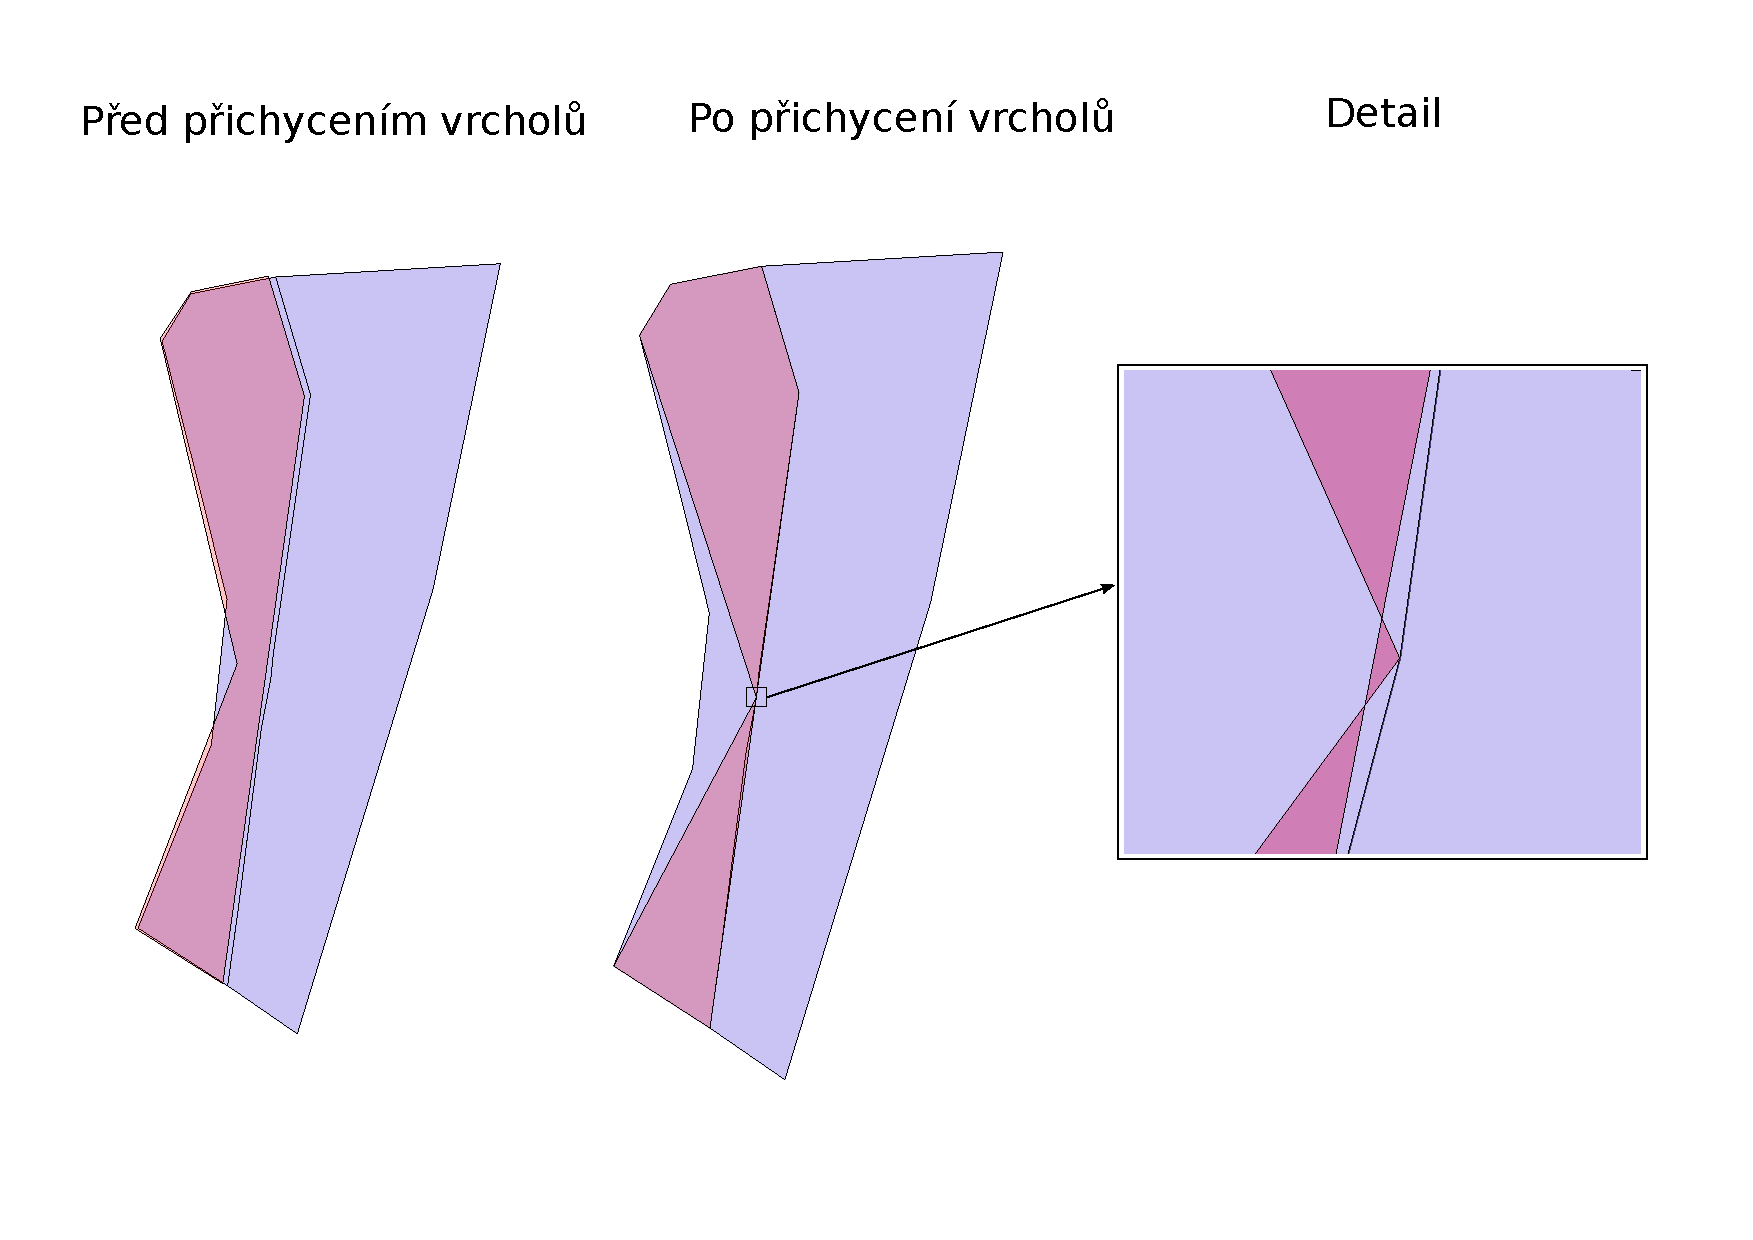
\includegraphics[width=350pt]{./pictures/vs-invalid.pdf}
      \caption{Vznik nevalidní geometrie při přichycení vrcholů}
      \label{fig:vs-nevalidni}
  \end{figure} 

Tyto chyby je samozřejmě možné opravit ručně po~zpracování. Avšak
v~rozsáhlých datasetech může být nevalidních prvků poměrně velké množství.
Pokud se toto nestalo z~důvodu nevhodného nastavení zpracování, bylo by 
vhodné, aby samotný algoritmus tyto chyby minimalizoval. To by bylo možné 
například přidáním nových vrcholů na~vhodná místa (dlouhé segmenty bez vrcholu
apod.). Další možností je zrušit přichycení vrcholu, pokud při něm vznikne
nevalidní geometrie. Nevýhoda takového postupu je horší zarovnání výsledné 
vrstvy. 

\subsubsection{Přichycení do jednoho bodu}
Speciálním případem vzniku nevalidní geometrie je situace, kdy se všechny 
vrcholy prvku přichytí pouze k~jednomu bodu. Tím vzniká z~linie či polygonu
bodový prvek. K~této situaci dochází v případě volby velké toleranční 
vzdálenosti v~poměru k~velikosti prvku. U~datasetů obsahujících prvky
o~výrazně rozdílných velikostech se tomu nelze vždy vyhnout. V~knihovně
\textit{GEOC} tento problém zatím není vyřešen. Nejjednodušší řešení, které
by bylo možné implementovat je nabídnout uživateli, co s~takovými prvky provést.
Na~výběr by byly tyto možnosti:
\begin{itemize}
 \item odstranění takových prvků,
 \item export těchto prvků do nové vrstvy, kde by bylo možné je dále upravovat,
 \item ponechání původní geometrie. 
\end{itemize}


\section{MatchingGeometry}
\label{problemy-mg}

Algoritmus \texttt{MatchingGeometry} vyhledává odpovídající si geometrie tak,
že nejdříve nalezne blízké prvky k~dané geometrii a~pak testuje postupně všechny
tyto blízké prvky. Po nalezení prvního odpovídajícího prvku se už další prvky
netestují. To může způsobit, že je nalezen sice odpovídající prvek, avšak
nemusí to být ten, který je danému prvku podobný nejvíce. U~polygonových vrstev
při vhodné volbě toleranční vzdálenosti tento problém většinou nenastává, 
ale u~vrstev liniových se může objevit poměrně často. 

Řešením by bylo seřadit před testováním blízké prvky dle nějakého
kritéria, které by určovalo pravděpodobnost, že si budou odpovídat. Takové
kritérium je však obtížné určit. U~polygonů by to mohla být velikost plochy,
kde se polygony nepřekrývají. Jak už bylo řečeno, nastává tento problém
spíše u~vrstev liniových, a~proto by takové kritérium příliš nepomohlo.
%Nejvhodnější by proto bylo použít pro liniové vrstvy zcela odlišný algoritmus.

% jeden prvek odpovídající dvěma

Výše uvedeným problémům u~liniových vrstev se lze vyhnout použitím jiného
algoritmu \textit{RoadMatcher/LineMatcher}, který porovnává pouze jednotlivé
úseky linií, nikoli celé prvky. 
% obrázek kritéria pro polygony   
% obrázek u linií

\section{CoverageAlignment}
\label{problemy-ca}

\subsubsection{Vytvoření trojúhelníkové sítě}
Po~nalezení odpovídajících si prvků je nutné určit vrcholy triangulační sítě.
V~použitém algoritmu jsou zvoleny dvojice blízkých vrcholů dvou odpovídajících
si prvků. Důsledkem tohoto výběru může být nepravidelné rozložení vrcholů sítě
a~také vytvoření troj\-úhelníkové sítě pouze nad~malou částí území, a~tudíž 
nezahrnující všechny odpovídající si prvky.
% obrázek tinu bez rohů a s rohy, kdy je výhodný

Pro pokrytí větší části území byly proto zahrnuty do~vrcholů rohové body, jejichž
souřadnice odpovídají extrémním souřadnicím ze~všech vrcholů prvků zpracovávané 
vrstvy, ke~kterým byl nalezen ekvivalent ve~vrstvě referenční. Tyto body mají 
v~obou systémech pro~transformaci totožné souřadnice. Tímto postupem se nejen 
zajistí zpracování všech odpovídajících si prvků, ale také zarovnání prvků 
i~v~případech, kdy se jako odpovídající určí pouze jeden či dva body, z~nichž 
by bez této úpravy nebylo možné TIN sestrojit. Nevýhodou zvoleného řešení jsou 
nevhodné tvary trojúhelníků na okrajích sítě a~tím způsobené méně přesné zarovnání 
v~těchto oblastech. Avšak i~přes tyto nevýhody jsou výsledky zarovnání datasetů 
s~použitím rohových bodů přesnější. 
% obrázek, kdy rohy mohou způsobit problémy

Vylepšením tohoto řešení by mohlo být použití bodů konvexní obálky pasujících
prvků namísto pouze čtyř rohových bodů.
% zjednodušení TINu -> odkaz na http://mapcontext.com/autocarto/proceedings/auto-carto-8/pdf/pages641-650.pdf

Velký vliv na~tvar TINu má způsob volby blízkých bodů. V~některých programech
(např. ArcGIS) je proto tento krok přenechán uživateli. Počet dvojic bodů je
sice obecně nižší, avšak jsou tak zvoleny pouze skutečně si odpovídající body
a~jejich rozložení je většinou pravidelné. Výsledek je pak blíže skutečnosti
než automatické zpracování. Navíc bylo experimentálně zjištěno, že větší počet
trojúhelníků nezajistí větší přesnost, a~obecně tak postačí jedna dvojice
bodů pro padesát prvků. % odkaz http://mapcontext.com/autocarto/proceedings/auto-carto-8/pdf/pages641-650.pdf nebo přímo Saalfeld

\subsubsection{Nevalidní geometrie}

V~případě nevhodné konfigurace odpovídajících si trojúhelníků může v~důsledku
lokální transformace dojít ke~vzniku nevalidních geometrií. Této situaci by se
dalo předejít výpočtem jednoho transformačního klíče ze~všech blízkých bodů
vyrovnáním a~aplikací globální transformace. Tak by nevznikly neplatné geometrie,
ale snížila by se přesnost zpracování, až na~situace, kdy by mezi datasety byl
téměř konstantní posun, natočení a~změna měřítka u~všech prvků.

% doplnit obrázek

Tento problém úzce souvisí s~volbou toleranční vzdálenosti. Při dodržení pravidla
o~nejkratším segmentu  se mu lze téměř vyhnout (stále mohou vznikat nevalidní 
geometrie u~příliš úzkých, protáhlých tvarů apod.). 

%Pravděpodobně by bylo možné nevalidní geometrie automaticky opravit např. výměnou
%vrcholů způsobujících křížení hran. Nyní je oprava těchto geometrií ponechána 
%na~uživateli.

\subsubsection{Volba počtu iterací}

V~popisu algoritmu zmiňuji, že proces zarovnání může probíhat iterativně.
Otázkou je volba počtu iterací. Nabízí se tři možnosti.
\begin{enumerate}
 \item konstantní počet iterací
 \item ponechání volby počtu iterací na uživateli
 \item opakování procesu tak dlouho, dokud není splněna určitá podmínka
\end{enumerate}
Pevně daný počet není příliš vhodný, jelikož vůbec nezohledňuje výsledky
předchozí iterace. Vzhledem k~tomu, že běžný uživatel by pravděpodobně
obtížně určil vhodný počet iterací, zůstává třetí možnost. Tím vyvstává
problém zvolení vhodné podmínky. Může to být počet nových odpovídajících 
si prvků, počet nově nalezených dvojic bodů, počet zpracovaných prvků aj.
Dle [..]  obvykle postačí dvě až tři opakování, % odkaz na [Saalfeld] 
přičemž mezi jednotlivými cykly je vhodná kontrola operátora,
který by měl odstranit případné hrubé chyby. Zároveň navrhuje jako podmínku
počet nově nalezených odpovídajících si prvků. Cyklus se tedy opakuje,
dokud jsou nacházeny nové dvojice pasujících prvků. Tento postup je   % zatím ještě ne
v~knihovně \textit{GEOC} implementován bez možnosti kontroly mezi iteracemi. 


\section{Line Matcher}
\label{problemy-lm}

\subsubsection*{Navázání linií}
Při určování podobných segmentů v~rámci jedné linie nastává problém jejich
navázání. V~závislosti na~nastavení funkce mohou při napojení výsledných
segmentů vznikat na~linii nežádoucí \uv{zuby} (viz obrázek \ref{fig:toothpic}). % viz obrázek
Tento problém v~algoritmu nebyl vyřešen, jelikož nelze jednoduše rozhodnout, 
kdy se jedná o~nesprávný tvar linie a~kdy je výsledek takto korektní.
Aby nevznikaly pouze samostatné nenavazující segmenty, byly i~přes toto
riziko napojovány.

\label{toothpic}
  \begin{figure}[hbt]
    \centering
      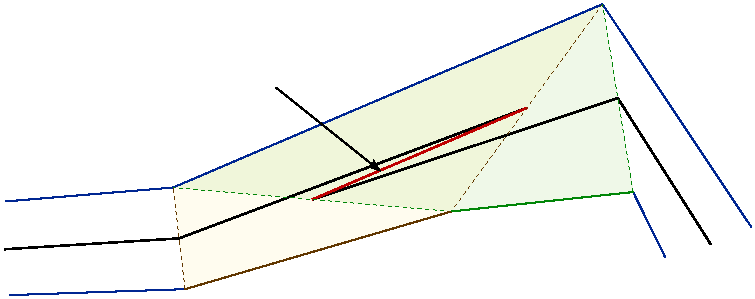
\includegraphics[width=300pt]{./pictures/tooth.pdf}
      \caption{Příklad situace, kdy vzniká \uv{zub}}
      \label{fig:toothpic}
  \end{figure}

\section{Automatická oprava nevalidních geometrií}
\label{problemy-opravy}

Jak již bylo uvedeno výše, častým problémem u~všech algoritmů je vznik
nevalidních prvků. Proto byla do knihovny \textit{GEOC} přidána třída
\texttt{Geometry\-Correction\-Operation}, kterou lze pro dodatečnou 
opravu nově vzniklých geometrií použít. Ne vždy je však jednoduché 
rozhodnout, jak geometrii změnit, aby výsledek odpovídal skutečnosti. 
V~programu proto byla aplikována jedna možnost způsobu opravy 
a~na~uživateli ponecháno rozhodnutí, zda automatickou korekci využít.

Automaticky je možné opravit tyto dvě chyby v~geometrii:

\begin{itemize}
 \item Křížení segmentů
	\subitem Změněna orientace hrany či hran mezi křížícími se úseky.
% obrázek
\label{crospic}
  \begin{figure}[hbt]
    \centering
      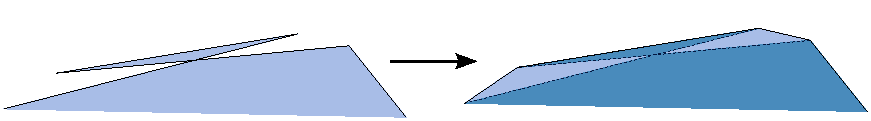
\includegraphics[width=300pt]{./pictures/crossing.pdf}
      \caption{Oprava křížících se segmentů}
      \label{fig:crossing}
  \end{figure}

 \item Slepé větve
	\subitem Vyřešeno odstraněním bodu na~konci větve.

\label{deadpic}
  \begin{figure}[hbt]
    \centering
      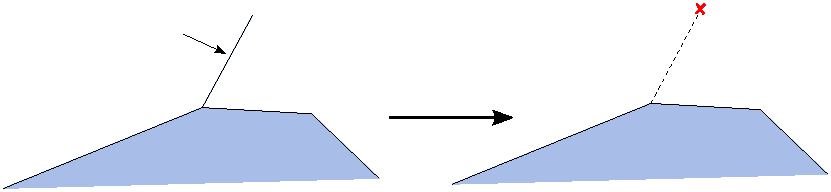
\includegraphics[width=300pt]{./pictures/dead-branch.pdf}
      \caption{Oprava slepých větví}
      \label{fig:dead-branch}
  \end{figure}
% obrázek
\end{itemize}

Samozřejmě existuje více možností, jak výše uvedené chyby opravit.
U~křížících se polygonů se často používá také pouhé přidání vrcholů
do~místa průsečíku segmentů. Tím vznikne validní geometrie a~nezmění
se přitom její tvar. Vzhledem k~tomu, že u~úprav prováděných 
s~polygony při slučování map, vznikají křížením většinou spíše drobné
\uv{výstupky}, je použité řešení přijatelné. Navíc funkci pro opravu
geometrií přidáním bodů obsahuje většina GIS programů, takže není
pro uživatele složité je po~spojení dat v~rámci \textit{postprocessingu}
aplikovat.
